\documentclass{article}
\usepackage[T1]{fontenc}
\usepackage{lmodern}
\usepackage{graphicx}
\usepackage{amsmath,amssymb}
\usepackage[a4paper,margin=2cm]{geometry}
\usepackage[absolute,overlay]{textpos}
\setlength{\TPHorizModule}{1mm}
\setlength{\TPVertModule}{1mm}
\usepackage[indonesian]{babel}
\usepackage{hyperref}
\setlength{\emergencystretch}{2em}
% unit: Halaman 20

\begin{document}

% === Halaman 20 (llm) ===

\vspace{231.66mm}

\begin{itemize}
    \item Demo online enkripsi ElGamal: \url{https://www.debjitbiswas.com/elgamal/}
\end{itemize}

\vspace{10mm}

% deskripsi: Screenshot dari ElGamal Encryption Playground yang menunjukkan proses enkripsi dan dekripsi antara Alice dan Bob, termasuk input prime p, generator g, private key, serta rumus matematika untuk perhitungan h, c1, c2, s, dan m.
% bbox normalisasi: [0.0900, 0.1300, 0.9300, 0.9100]
\begin{textblock*}{176.40mm}(18.90mm,38.61mm)
\noindent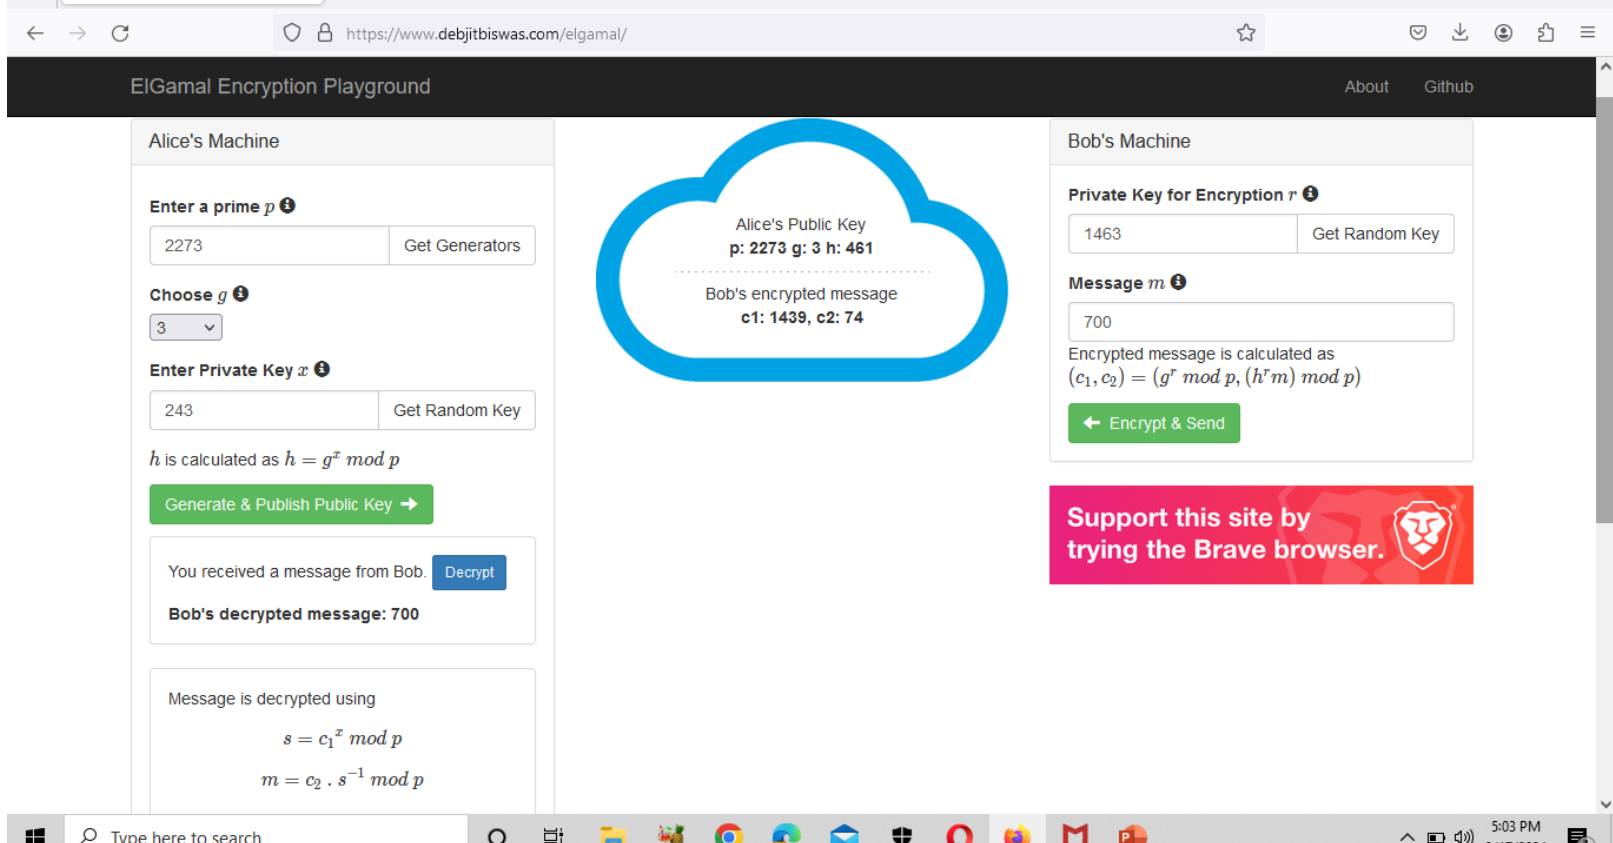
\includegraphics[width=176.40mm,height=231.66mm]{../../images/llm/page_020_img_01.png}%
\end{textblock*}

\end{document}
